\chapter{Tâche~7: Activités de terrain}

\section{Plant de production d'ammoniac à Tertre}
Dans le cadre de notre projet P3 nous sommes partis visiter le plant de production de Yara à Tertre. Cette petite excursion nous a permis de visualiser le fonctionnement global et les différentes étapes de la fabrication de l'ammoniac. Le directeur de l'entreprise nous a été présenté et nous a expliqué son rôle d'ingénieur chimiste dans la gestion du plant. Après une présentation de la partie chimique et énergétique du procédé, ainsi que des éventuels problèmes de sécurité, nous avons découvert le site-même de la production. Dans ce rapport, nous avons résumé les informations nouvellement acquises durant cette journée qui nous semblaient utiles pour la réalisation du projet. Nous n'avons donc pas repris les informations disponibles dans notre premier rapport.
\subsection{Partie chimique et énergétique}
\textbf{Primary reformer (1000\,\degree C)}
\begin{itemize}
\item Mélange gaz/vapeur qui descend dans des tubes chauffés par 180 brûleurs au gaz naturel.
\item Formation de \ce{H2} qui remonte dans un autre tube et est guidé vers le secondary reformer.
\item L'excès de vapeur d'eau est requis sinon le méthane se «craque» lui-même avec la chaleur et crée de la pierre, qui s'accumule dans les tuyaux et les bouche. (Il existe un système de contrôle indépendant.)
\end{itemize}

\textbf{Secondary reformer }
\begin{itemize}
\item Ajout d'air, ce qui augmente la température par inflammation.
\item Comme la réaction est endothermique, la réaction est favorisée.
\end{itemize}

\textbf{Décarbonatation}
\begin{itemize}
\item Absorbeur sous pression alimenté par une solution d'amine (qui absorbe bien le \ce{CO2}).
\item Absorbe le \ce{CO2} dans la solution et le libère ensuite dans les strippers.
\end{itemize}

\textbf{Méthanateur}
\begin{itemize}
\item Il reste du \ce{CO} et du \ce{CO2}, donc on refait la réaction inverse du primary reformer.
\item On utilise une partie du \ce{H2} pour les éliminer.
\item On peut récupérer le \ce{CH4} produit au reformage primaire.
\end{itemize}


\textbf{Compresseur}
\begin{itemize}
\item Augmentation de la pression de $27\,\bbar$ à $130\,\bbar$.
\end{itemize}

\textbf{Synthèse \ce{NH3}}
\begin{itemize}
\item Réaction: $\ce{N2 + 3H2  -> 2NH3}$ avec $\Delta H = -45.6\,\kilo\joule\per\mole$ (exothermique).
\item Energie de dissociation: $946\,\kilo\joule\per\mole$ à $1000\,\celsius$.
\item Utilisation de catalyseurs pour diminuer l'énergie d'activation de la réaction sans changer le chemin réactionnel.
\item L'énergie d'activation est l'énergie à apporter pour démarrer la réaction, même si elle est exothermique.
\item Le refroidisseur entre les deux convertisseurs refroidit le mélange pour que l'équilibre de la réaction se déplace vers la droite.
\item Le condensateur condense l'ammoniac à $-33\,\celsius$; en fin de boucle il y a
14 \% d'ammoniac.
\item Le reste du mélange part en recyclage en passant par un stockage pressurisé qui amène à une purge pour éviter l'accumulation d'argon.
\item La production de chaleur en théorie est de $30\,\giga\joule$ par tonne de \ce{NH3}, mais en pratique on obtient $20\,\giga\joule$ par tonne de \ce{NH3}.
Cette différence est expliquée par le fait qu'il y a une purification de \ce{NH3}.
\end{itemize}

\subsection{Sécurité}

\textbf{Composés à risque}
\begin{enumerate}
\item Azote : $\ce{N2}$
\begin{itemize}
\item Compose 78,08 \% de l'air
\item Inodore et incolore 
\item Risques de suffocation très rapide, donc dangereux dans des espaces confinés
\item Demande une grande quantité d'énergie pour être dissocié
\end{itemize}
\item Hydrogène : \ce{H2}
\begin{itemize}
\item Extrêmement explosif
\item Extrêmement volatile (même à travers certains métaux, donc problème de matériaux)
\item Problèmes de corrosion dans les réacteurs, dus à la réaction
\ce{Fe3C + 2H2 <=> CH4 + 3Fe}.
Cette réaction produit du fer pur, ce qui va introduire de la rouille dans le réacteur.
\end{itemize}

\item Ammoniac : \ce{NH3}
\begin{itemize}
\item Incolore mais très odorant
\item Plus léger que l'air
\item Température critique élevée ($132.4\,\celsius$), donc facile à liquéfier
\item Stable à température normale
\item Explosif en présence d'air
\item Réagit très rapidement avec l'eau
\end{itemize}
\end{enumerate}

\textbf{Organisation pratique}

Durant notre visite, il nous a été conseillé de porter un casque et aussi de garder sur nous un masque afin que nous ne respirions pas de gaz toxiques au cas où il y aurait une fuite. Nous avons fait un bref passage à la «tour de contrôle» qui détecte à l'aide d'un système informatique des fuites ou autres problèmes dans les réactions chimiques. Ce fut impressionnant de voir tous ces écrans et nous nous sommes rendus compte du nombre de réactions et de différents paramètres à prendre en compte.

\textbf{Considérations environnementales}
\begin{itemize}
\item $500\,\ton$ de \ce{CO2} sont rejetées par jour, le reste étant liquéfié et revendu à des entreprises produisant des boissons gazeuses.
\item La solution d'amine est meilleure que l'arsenic (poison) ou les potasses (énergivores et corrosives) utilisés dans d'autres entreprises.
\item Les fumées du primary reformer doivent être récupérées.
\item L'huile usagée des parties mobiles doit aussi être récupérée.
\end{itemize}
Une manière de diminuer l'impact sur l'envirronement est de
travailler sur le design et l'efficacité de la production,
et donc de maîtriser le processus.

\subsection{Conclusion}

Cette visite fut très enrichissante pour nous car elle nous a tout d'abord aidés à visualiser notre projet. Grâce à cette visite, nous avons pu voir en réalité tout ce qu'on avait traité en séance de projet.
Et, tout aussi important, nous découvert à quoi ressemblait la vie d'un ingénieur chimiste dans une usine de production, dont nous avons retenu les compétences-clés : «Dans ce métier, il faut proposer des solutions, optimiser, être créatif et critique, et surtout, avoir de l'imagination!» 

\section{Total Research Technology à Feluy}
Nous avons commencé la matinée par une conférence où l'on nous a expliqué le fonctionnement général de Total. Ensuite, nous avons pu visiter plusieurs lieux stratégiques du site, tels que le lieu de fabrication des granulés de polypropylène, la salle de contrôle des unités-pilotes ou encore un laboratoire.
Voilà les informations que j'ai pu recueillir lors de cette matinée qui peuvent nous intéresser dans le cadre du projet :
\subsection{Sécurité}
La sécurité est, bien évidemment, la priorité absolue de Total, car si un accident devait arriver, ce serait sûrement annonciateur d'au minimum la fermeture du centre. Tout autant la sécurité des personnes que des installations et du matériel sont importantes. Les procédures sont donc extrêmement strictes et réglementées, et on doit rapporter chaque incident, peu importe sa gravité.
\begin{itemize}
\item Pour ne pas devoir effectuer les tests sur l'usine principale, Total a mis au point des unités-pilotes, qui sont en quelque sorte de petites usines de taille réduite.  Les travailleurs de la salle de contrôle nous ont expliqué que la corrélation entre les résultats obtenus dans l'unité-pilote et dans l'usine principale était vraiment bonne et fiable.
\item Le laboratoire est une sorte « d'unité-pilote de l'unité-pilote », qui permet de faire des tests à une échelle encore plus petite.
\end{itemize}

\subsection{Contrôle de qualité des procédés}
Les unités-pilotes, et plus principalement le hall des applications, que nous avons eu la chance de visiter, permettent de produire des échantillons à livrer aux clients avant approbation de ceux-ci, ou encore d'effectuer des tests. Ainsi, il n'y a pas besoin de faire tourner l'immense usine juste pour quelques kilos d'échantillons; ou de reconfigurer toute la chaîne si l'on veut changer une seule chose dans le produit.

\subsection{Recyclage}
Dans le temps, Total brûlait dans des énormes torchères, au « flare », les rejets de gaz. Maintenant, ils recyclent tout, ce qui est bien plus écologique. Ainsi, il est dorénavant assez rare de voir les torchères d'une raffinerie émettre des flammes.

\subsection{Pression dans les réacteurs}
Les travailleurs de la salle de contrôle nous ont dit que les réacteurs de l'unité-pilote étaient conçus pour résister à des pressions pouvant aller jusqu'à $100\,\bbar$, mais en général, la pression ne dépasse pas les $60\,\bbar$.

\section{Unité de biométhanisation à Tenneville}

Nous avons été visiter l'unité de biométhanisation sur le site de Tenneville dans la
province du Luxembourg. Elle appartient à deux intercommunales, BEP et AIVE, dont
l'activité est centrée sur l'environnement, respectivement dans les provinces de Namur
et du Luxembourg. Le rôle de cette unité est de revaloriser les déchets ménagers
organiques (environ $30\,000$ tonnes par an) provenant de ces deux provinces en les
transformant en compost et en bio gaz, celui-ci utile pour produire de l'électricité et de la
chaleur.

\subsection{Description du système}

\begin{figure}
\centering
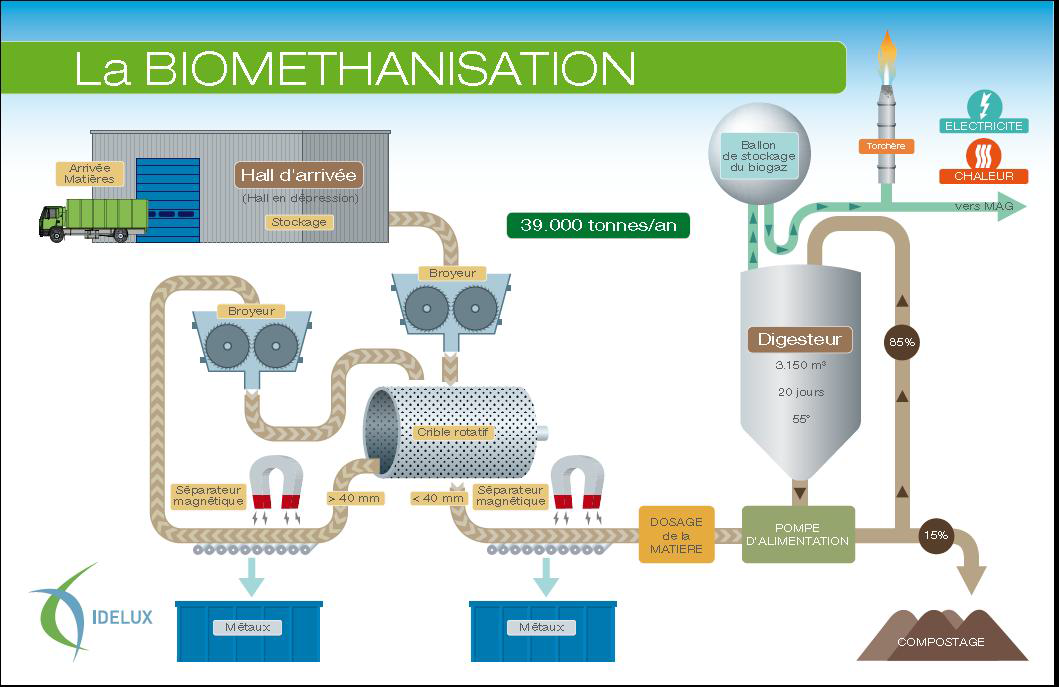
\includegraphics[width=0.9\textwidth]{img/biometh1}
\caption{Système complet d'une usine de biométhanisation. (Source : IDELUX)}
\label{fig:biometh1}
\end{figure}

Le système complet est illustré dans la figure~\ref{fig:biometh1}.
Lorsque les déchets arrivent, ils sont tout d'abord contrôlés pour éviter toute contamination, de type radioactive par exemple. Ils sont ensuite amenés vers des broyeurs qui vont les déchiqueter et en retirer les sacs plastiques. Environ 10\% des déchets seront rejetés et ne passeront pas à l'étape suivante. Cette dernière consiste en un tambour qui va laisser passer les morceaux les plus fins. Par la suite, un séparateur magnétique va en extraire les métaux. La masse de déchets organiques est alors prête pour aller dans le digesteur. C'est là que la vraie biométhanisation commence. « Tout est naturel », comme le disait notre guide. Il ne faut donc rien y ajouter pour que les réactions se fassent, si ce n'est de l'eau et de la chaleur car la réaction est endothermique. La température y est maintenue autour de $40\celsius$. Il est également nécessaire de vérifier que le rapport de carbone sur azote soit d'environ 30 à 35.

\begin{figure}
\centering
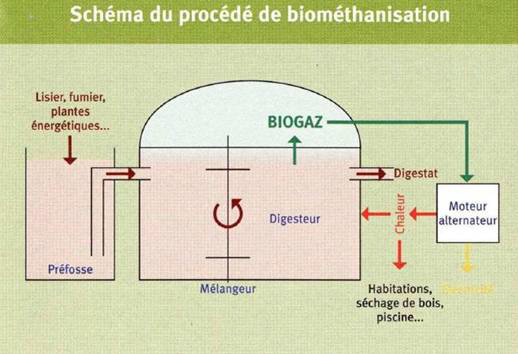
\includegraphics[width=0.9\textwidth]{img/biometh2}
\caption{Schéma du procédé centré sur la digestion. (Source : Vade-mecum technique et administratif relatif à la biométhanisation de biomasse humide en Région wallonne)}
\label{fig:biometh2}
\end{figure}

Dans le digesteur (figure~\ref{fig:biometh2}), en l'absence d'air, ce sont alors différentes bactéries et levures qui vont opérer. Il y aura tout d'abord une dégradation enzymatique par les bactéries. Ensuite, l'acidogenèse qui consiste à transformer ces chaines courtes en acides gras et \ce{H2}, et l'acétogénèse, durant laquelle les métabolites vont permettre la production d'acétate. Puis les bactéries acétotrophes et acidotrophes vont produire le \ce{CH4} et \ce{CO2}. Au final, on retrouvera dans le biogaz environ $55\%$ de méthane (\ce{CH4}) et $43\%$ de dioxyde de carbone (\ce{CO2}). Le reste est ce qui n'aura pas été utilisé par les bactéries ainsi que du sulfure d'hydrogène (\ce{H2S}). Si ce reste ne porte pas vraiment à conséquence, il faut tout de même être plus prudent avec le \ce{H2S} qui peut être très toxique. Il sort environ 114 litres de biogaz par $\kilogram$ de déchets frais amené au centre.

Grâce à une pompe, les matières organiques sont à chaque fois introduites par le haut dans le digesteur et on récupère ce qui a macéré et eu le temps de réagir par le bas. Cette masse est appelée le digestat. C'est ce qui va être transformé en compost. Il faut encore la sécher. De novembre à mars, pendant la période plus froide, cela devient plus difficile de sécher cette matière et cela entraine un mauvais rendement. Ils rajoutent donc $5\%$ à $10\%$ de chaux pour une structure plus alvéolaire qui favorise ainsi le passage de l'air et le séchage. Ensuite, cette masse, en attente de compost, va reposer sur des dalles sous lesquelles soufflent de grand ventilateur pour l'alimenter en oxygène et la refroidir. Une fois fini, le compost pourra être utilisé comme engrais dans l'agriculture.

Quant au biogaz, ils ont décidé de ne pas le transformer en carburant mais, grâce à des moteurs, en électricité et chaleur. L'électricité alimente les machines du site et le reste est revendu sur le réseau, ce qui alimente 1500 ménages de la région. La chaleur est également réutilisée par l'unité elle-même pour le séchage des boues, la chaleur à apporter au digesteur et le chauffage des locaux. Sur les 8 à 9 millions de $\kilo\watt\hour$ de chaleur produits par an, ils en utilisent que 5 à 6. Et, tout le biogaz qui n'est pas utilisé doit être brulé car ils n'ont pas le droit de le relâcher tel quel dans l'atmosphère.

\subsection{Environnement}
Cette unité de biométhanisation est un exemple en matière environnementale.
Tout d'abord par son rôle premier qui est de revaloriser des déchets ménagers plutôt que de les enfuir directement dans le sol. Elle crée ainsi un engrais biologique bien meilleur pour les cultures que les engrais chimiques qui ont été utilisés sur les terres wallonnes et les ont mis dans un état critique. Et elle produit également de l'énergie verte.

De plus, en étant autonome énergétiquement, elle n'utilise pas d'énergie fossile et il n'y a pas non plus d'énergie perdue dans le transport de celle-ci. C'est économiquement et écologiquement avantageux et durable.

Enfin, leurs eaux usées sont directement utilisées par une usine de recyclage de bâches agricoles qui est venues s'installer juste à côté du site. Ainsi, ils peuvent effectuer leur premier rinçage sans gaspiller de l'eau propre.

\subsection{Lien avec notre projet}
Nous avons cherché à faire des liens entre cette visite et notre projet. Bien que les procédés chimiques qui se produisent au sein de cette unité n'ont pas de rapport avec ceux étudiés pour la synthèse de l'ammoniac, nous pouvons reprendre leurs idées de proximité pour réduire l'impact environnemental. En effet, nous avons, au cours du procédé de la synthèse d'ammoniac, également des éléments « déchets » qui pourraient peut-être intéresser d'autres usines.


Ensuite, l'unité de biométhanisation produit en grande quantité du méthane, composé que l'on souhaite utiliser dans nos propres procédés pour obtenir l'hydrogène nécessaire à la synthèse de l'ammoniac. Une question qu'on se pose alors est : « Serait-il possible d'utiliser le méthane produit ici dans notre projet ? »


Si l'on voulait utiliser le méthane, il faudrait tout d'abord le séparer du reste du gaz pour le rendre pur et utilisable. Des méthodes ont déjà été mises au point, comme la séparation par membrane. Evidemment cela a un coût.
Mais, pour le moment, l'exploitation du méthane pour autre chose que la production d'électricité ou de chaleur n'est pas du tout à l'ordre du jour à Tenneville. « À quoi cela sert-il de vouloir produire de l'ammoniac avec notre méthane, puisque l'ammoniac sert en grande partie à faire de l'engrais et que nous, nous produisons un bon engrais biologique », nous a répondu le guide quand nous avons évoqué cette possibilité. Plus qu'un problème de mise en pratique ou financier, cela s'avère aussi peu compatible avec l'idéologie environnementale de l'usine.

\section{Laboratoire d'électrolyse}
Dans le cadre du projet P3, nous avons pu participer à un laboratoire dans le but de comparer différentes techniques de production de dihydrogène. Le procédé que nous utilisons est le vaporeformage, mais pour mieux justifier son usage, nous avons eu l'occasion de tester un autre procédé : l'électrolyse de l'eau.

\subsection{Expérience}
L'électrolyse de l'eau est une réaction d'oxydo-réduction au cours de laquelle l'eau est décomposée en dihydrogène et en dioxygène, grâce à un courant électrique envoyé entre deux électrodes (anode en plomb et cathode en cuivre) plongées préalablement dans l'eau (voir figure~\ref{fig:electrolyse}).
\begin{figure}
\centering 
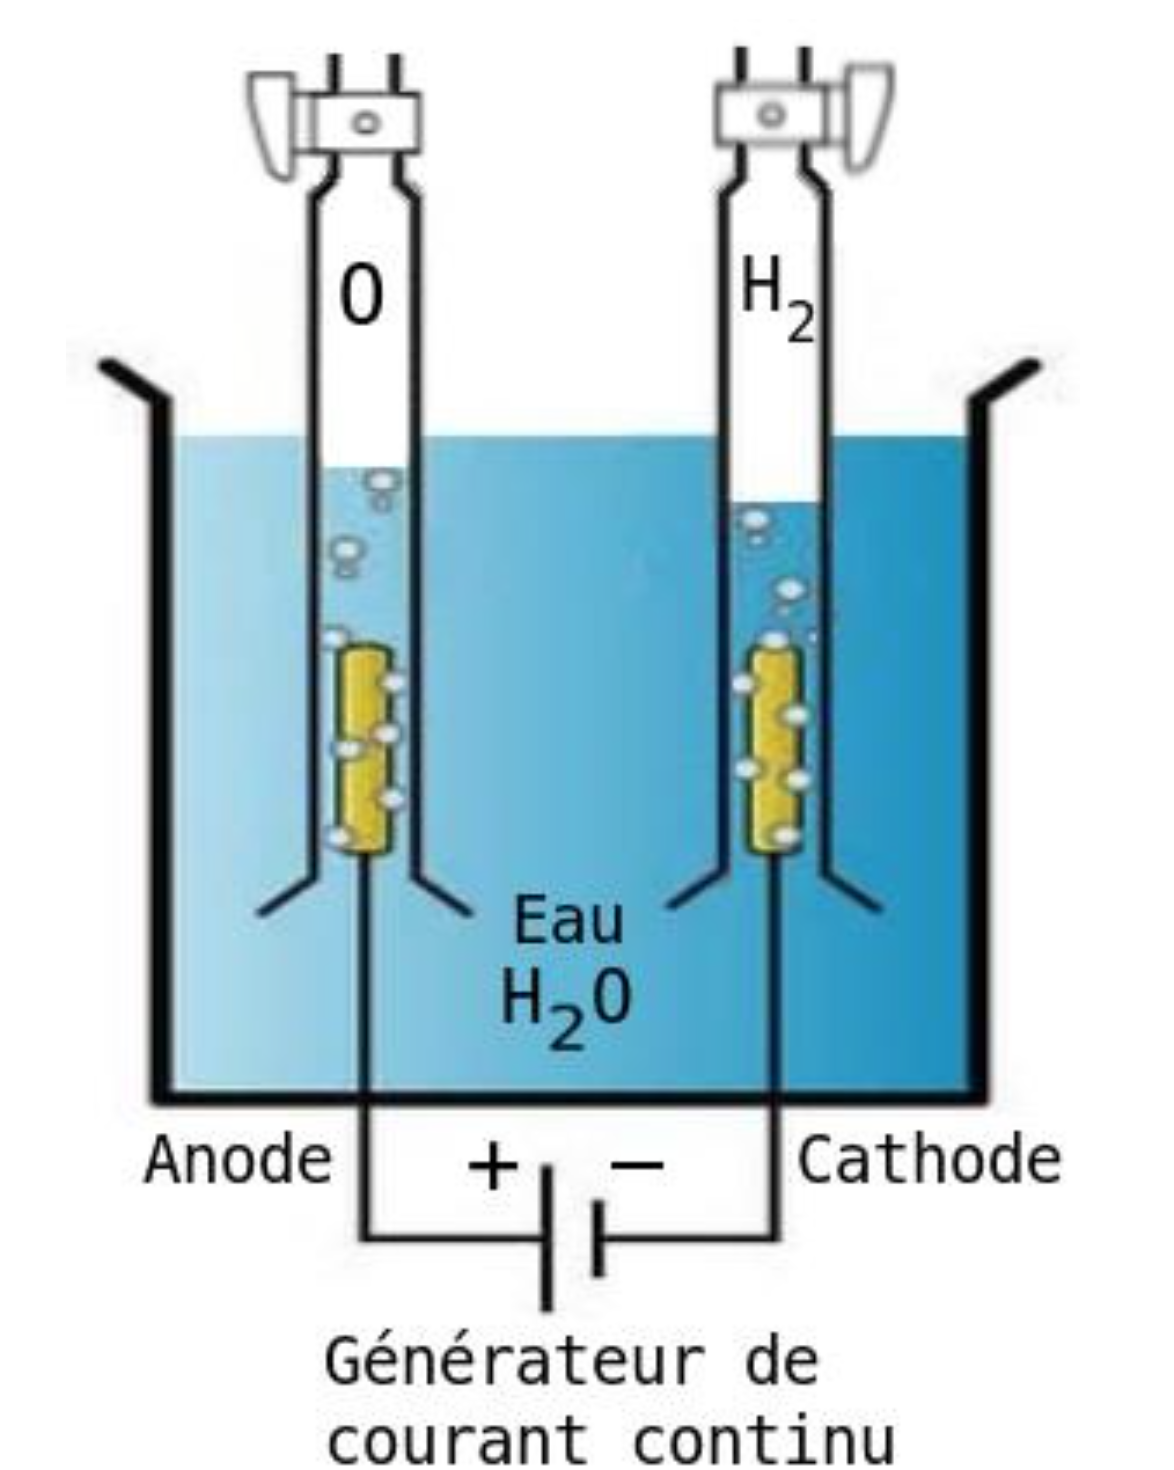
\includegraphics[width=0.4\textwidth]{img/p1}  
\caption{Procédé d'électrolyse de l'eau. \cite{energie-renou}} 
\label{fig:electrolyse}
\end{figure}

Dans notre expérience nous avons dilué du sulfure d'hydrogène dans l'eau pour pouvoir en faire varier le pH. Ensuite, nous avons observé l'évaporation du dihydrogène en fonction du temps, pour les différents pH testés. Finalement nous avons également changé le courant qui passe dans les électrodes, de $0.5\,\ampere$ à $1.0\,\ampere$.

\subsection{Résultats}

\begin{figure}
\centering
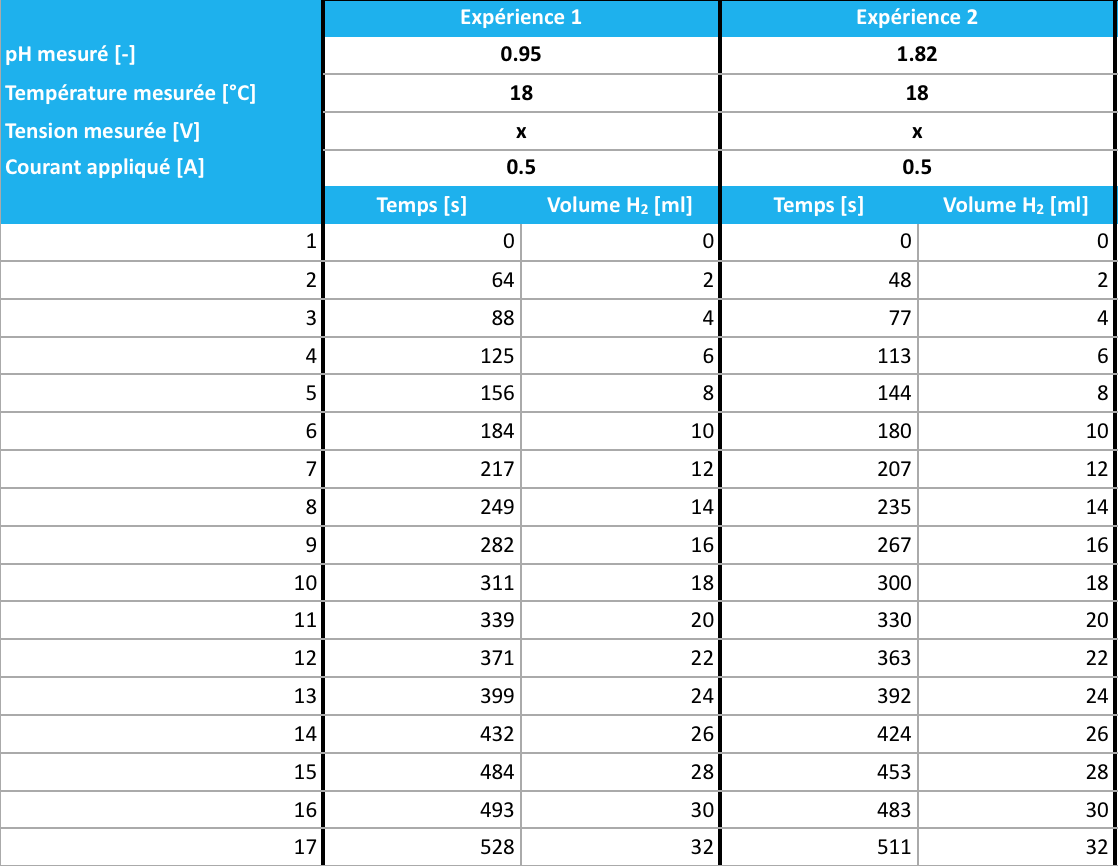
\includegraphics[width=0.8\textwidth]{img/p2}
\caption{Résultats pour un pH de $0.95$ et un pH de $1.82$, à $0.5\,\ampere$}
\label{fig:elec-results1}
\end{figure}

\begin{figure}
\centering
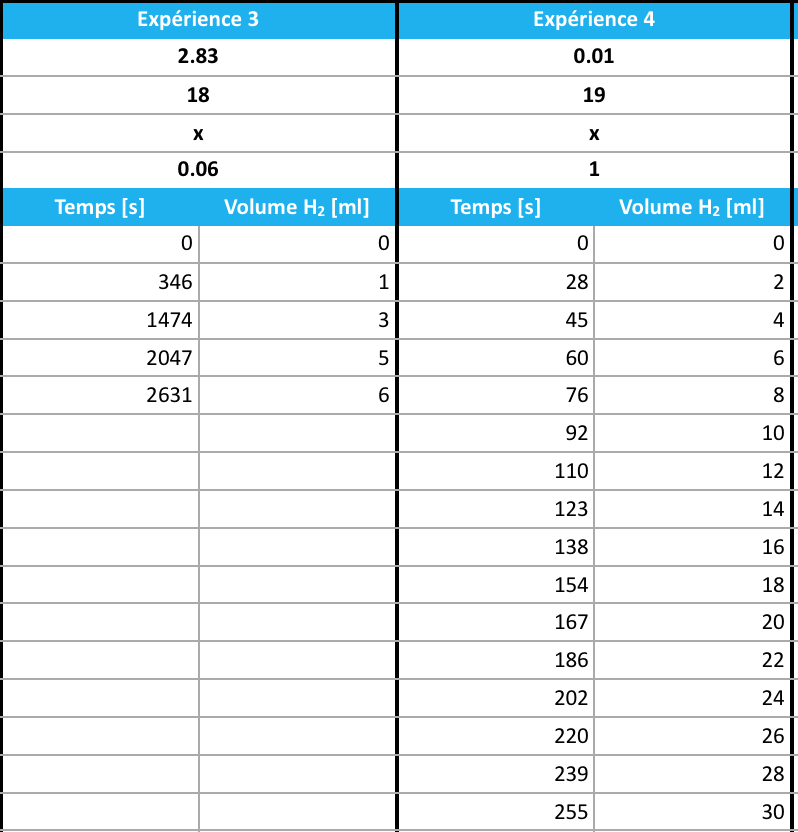
\includegraphics[width=0.6\textwidth]{img/p3}
\caption{Résultats pour un pH de $2.83$ à $0.06\,\ampere$ et un pH de $0.01$ à $1.0\,\ampere$}
\label{fig:elec-results2}
\end{figure}

Nous mesures sont reprises dans les figures~\ref{fig:elec-results1}
et~\ref{fig:elec-results2}.
Nous remarquons que plus la solution est acide, plus l'évaporation est rapide. Nous avons également observé qu'a partir d'un certain pH, il y a saturation du courant, et donc le dégagement de dihydrogène (et d'oxygène) est limité et prend beaucoup plus de temps.

\subsection{Avantages et inconvénients}
L'avantage principal de cette technique est son aspect écologique, en effet on pourrait arriver à la réaliser sans émettre (ou très peu) de dioxyde de carbone (en utilisant par exemple les éoliennes pour générer du courant). Cependant, son inconvénient majeur est son faible rendement (80\% environ) ainsi que son coût de production, au moins 3 fois plus élevé que celui du vaporeformage. \cite{wehicles-elec}

Aujourd'hui c'est le vaporeformage qui est principalement utilisé (de part son prix attrayant et son rendement élevé), mais à l'avenir, en raison de son impact sur l'environnement et de l'épuisement des énergies fossiles, il faudra développer des techniques plus écologiques. \cite{wehicles-vapo}

\section{Atelier créatif}
Dans le cadre du projet, une partie des activités proposées concernait la production créative à adopter au sein d'un groupe de projet afin de mener à bien les objectifs qui doivent être réalisés.

Tout d'abord, au sein même d'un groupe, chacun est considéré comme créatif, il n'y a pas d'élus. Chacun peut s'exprimer comme il l'entend dans un processus qui se veut dynamique, stimulant et structurant. Le but étant d'aboutir à des solutions inédites, originales et pertinentes.
Quatre rôles clés ressortent dans un même groupe : le clarificateur, l'idéateur, le développeur et le réalisateur.

La clarificateur va clarifier le problème, poser la problématique et l'identifier afin que le groupe aie la bonne question sur laquelle partir afin de baser leur réflexion. L'idéateur va donner toutes les idées qui lui passent par la tête, peu importer leur pertinence, il ne néglige rien. Le développeur, quant à lui, va rebondir sur les idées farfelues, afin de pousser la réflexion plus loin. Enfin, le réalisateur, va traiter l'information, aller plus vite pour faire une synthèse.

Dans la recherche d'une solution, il faut aussi chercher la contradiction dans le but de trouver des solutions efficaces. La question de la la problématique posée, il faut ensuite la démonter et non foncer directement vers une solution.
Deux modes de pensée sont à adopter : les modes de pensée divergent et convergent. D'un côté la divergence avec la recherche de quantité. On liste tout ce qui nous passe par la tête, on suspend le jugement. De l'autre côté, il y a cette idée de convergence, on converge vers quelque chose de plus précis, se rapprochant de la solution au problème posé.

Lors de ce processus, il est important que le groupe mette un plan d'action en oeuvre. Mais avant toute communication, il faudra vérifier que chacun des membres du groupe adhèrent à la solution. Quatre étapes clés sont présentes lors de ce dernier processus :
\begin{itemize}
\item La mise en évidence des attentes (\emph{insight}) : les besoins du clients
\item La réponse de l'entreprise (les promesses) : ce qu'on va envoyer au groupe des décideurs, la réponse apportée au besoin.
\item La démonstration technique (raison d'y croire) : adopter notre langage au public auquel nous allons expliquer les résultats.
\item La base line (\emph{claim}) : le slogan, finir de sorte que la réponse apportée soit mémorisée par le public ciblé.
\end{itemize}

Plusieurs remarques ont été relevées quand à la vision du système industriel de nos jours et vers quel nouveau système nous devrions évoluer.
Les valeurs de notre système actuel telles que le progrès, la croissance, la compétition, le temps (qui vaut de l'argent), la quantité (toujours et encore plus) ou encore l'homme séparée de la nature, sont en crise. Ces valeurs ont engendré un impact négatif sur l'habitation, le travail, l'alimentation et l'agriculture, l'énergie, l'environnement, la science, la mobilité ou encore la santé. La croissance a mené à un étouffement. Il nous faut donc muter vers un développement durable.

Un valeur importante à apporter est la culture du \emph{care}, c'est-à-dire du «prendre soin», d'avoir de l'intérêt en le sens des choses. Il faut arrêter de détruire et régénérer.
Il faut tendre vers l'interdépendance, repenser la dépendance que l'on a vis-à-vis des autres, de passer de compétition à collaboration avec le vivant. En effet, seul on va plus vite mais ensemble on va plus loin.

C'est donc dans cette optique que nous devons évoluer et penser tout au long de ce projet.
